\chapter{Problem'atica}

Debido al crecimiento de Internet visto en el C'apitulo \ref{desarrolloWeb} y a los problemas que presenta el protocolo HTTP en su implementaci'on (visto en el C'apitulo \ref{protocolos}), se busca mejorar los tiempos de carga de los sitios web. 

%PONER PORQUE SE BUSCA MEJORAR LOS TIEMPOS DE RESPUESTA.

\section{T'ecnicas de optimizaci'on}

Es importante conocer d'onde es que el usuario pasa el tiempo esperando en la carga de un sitio web. Seg'un el estudio de Steve Souders en su libro \citep{highPerformanceWebSites}, el cliente tarda menos del 20\% para obtener el documento HTML, y el tiempo restante para recibir el resto de los componentes del sitio. Es importante enfocarse en el 80\%, 90\% restante, ya que el tiempo no se desperdicia en descargar el documento HTML ni en el procesamiento que realiza el servidor antes de enviarnos la petici'on. Esto se resume en la ''Regla de Oro de la Performance'' de dicho libro:

\begin{quote}

\textit{Solo el 10-20\% del tiempo de respuesta del usuario es consumido descargando el documento HTML. El otro 80-90\% se consume descargando todos los componentes de la p'agina.}

\end{quote}

Plantea 14 reglas para la optimizaci'on de los sitios que se describen a continuaci'on.

\begin{enumerate}

\item \textbf{Minimizar la cantidad de peticiones.}

La idea b'asica es eliminar las peticiones al servidor, esto se hace utilizando varias t'ecnicas enumeradas a continuaci'on.

	\begin{enumerate}
	\item Mapa de Im'agenes - Permite asociar m'ultiples 'areas en una imagen para que se puedan cliquear y realizar cierta acci'on (el ejemplo m'as b'asico es el de navegar un hiperv'inculo). En vez de utilizar m'ultiples im'agenes para realizar un men'u por ejemplo, se utilizar'ia una sola mapeada. De esta manera se ahorran las peticiones de las im'agenes por 1 sola petici'on.
	\item CSS Sprites - Permite combinar v'arias im'agenes en una sola, luego en el sitio, se define que parte de la imagen combinada desea mostrarse. Por ejemplo, en el sitio de Google cuando se realiza una b'usqueda, se utiliza el Sprite que se ve en la Figura \ref{css_sprites}.
		\begin{figure}[htbp]
		\begin{center}
			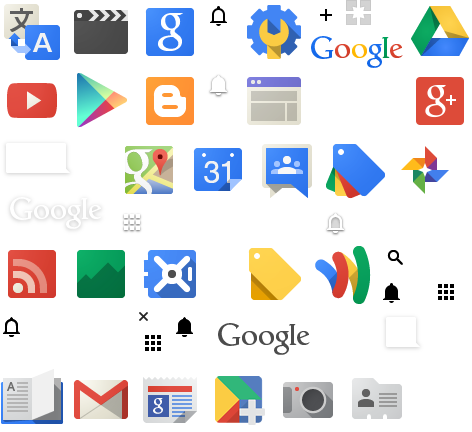
\includegraphics[width=150px]{img/css_sprites}
			\caption{\small Sprite del sitio www.google.com}
		\end{center}
		\label{css_sprites}
		\end{figure}

	A simple vista se ven 44 im'agenes combinadas. La utilizaci'on de este Sprite reducir'ia todas estas peticiones a 1 sola.
	\item Im'agenes Inline - Se pueden incluir im'agenes en un sitio web sin necesidad de realizar una petici'on al servidor definiendolas con el esquema \textit{data:} \ref{rfcData} dentro del c'odigo HTML de la p'agina.
	\item Combinar Scripts y Hojas de Estilo - Como la mayor'ia de los sitios actuales utilizan Javascript y CSS, es preferible que los Scripts se combinen en uno solo al igual que las Hojas de Estilo. En el caso de tener varios archivos, el navegador va a generar una petici'on por cada uno de ellos de no tenerlo almacenado en una copia local.
	\end{enumerate}
\item \textbf{Utilizar un CDN}

La proximidad del cliente al servidor web tiene un impacto en el tiempo de respuesta de las peticiones. No es lo mismo solicitar un recurso localizado China estando en Argentina que uno ubicado dentro del mismo pa'is. Por ende, si los contenidos est'an cerca\footnote{En t'erminos de distancia f'isica.} el tiempo de respuesta es menor. Debido a que solo el 10-20\% del tiempo de respuesta se dedica al HTML (visto al inicio de este cap'itulo), si el resto de los recursos del sitio se encuentran cerca del cliente, se mejorar'ian los tiempos de respuesta. Para esto es necesario dispersar estos recursos geogr'aficamente.

Un CDN\footnote{Content Delivery Networks} es una red de distribuci'on de contenidos. Son servidores dispersados geogr'aficamente que ofrecen r'eplicas de los recursos de un sitio particular para brindarlos al cliente desde el m'as cercano a su locaci'on.

Utilizar el servicio que brinda un CDN mejora los tiempos de respuesta de los usuarios.
\item \textbf{A'nadir Headers para Cach'es}

Cuando un usuario visita el sitio por primera vez, realiza tantas peticiones HTTP como recursos tenga la p'agina. Utilizando Headers Expires o Cache-Control\footnote{Desde HTTP 1.1} (Cap'itulo \ref{protocolos}, Secci'on \ref{headers}) se puede hacer que los recursos puedan ser almacenados en Cach'es (Cap'itulo \ref{cache}). Esto disminuye la cantidad de peticiones en una posterior visita a la p'agina del mismo usuario.

La performance del tiempo de respuesta del sitio mejora seg'un la cantidad de ''Hits''\footnote{Necesidad de solicitar un recurso que ya tengo almacenado en la Cach'e} que el usuario tenga de los componentes del sitio.
\item \textbf{Comprimir los componentes (Gzip)}

Se puede reducir el tiempo de respuesta, disminuyendo el tama'no de la respuesta HTTP. Esto se puede realizar comprimiendo el recurso que se est'a solicitando. La reducci'on del tiempo es mayor en ambientes en donde el ancho de banda es bajo. El formato \textit{Gzip}\footnote{http://www.gzip.org/} \citep{rfcGzip} es el m'as popular y el m'as efectivo, el otro formato que se usa con menos frecuencia es \textit{deflate} \citep{rfcDeflate}.

El usuario tiene que enviar en la petici'on un Header \textit{Accept-Encoding} indicando los m'etodos aceptados. Cuando el servidor recibe este Header, puede comprimir el recurso utilizando alguno de los m'etodos indicados por el usuario. Este devuelve la respuesta con un Header \textit{Content-Encoding} indicando el tipo de compresi'on utilizado en el recurso que se est'a enviando.

Los tipos de archivos que se deber'ian comprimir son aquellos de texto, tales como HTML, Scripts, CSS, etc. Aquellos formatos que ya se encuentran comprimidos como las im'agenes o los archivos PDF no deber'ian comprimirse ya que se desperdicia tiempo de CPU del servidor\footnote{Para realizar la compresi'on.} y adem'as puede incluso incrementar el tama'no del archivo.

\item \textbf{CSS en la parte superior del HTML}

Las Hojas de Estilo deben incluirse en la parte superior del HTML. De esta manera, los navegadores pueden ir renderizando la p'agina a medida que van llegando las respuestas de las peticiones. Esto es importante en t'erminos de usabilidad, para brindarle un medio visual \footnote{Carga progresiva del sitio.} al usuario que est'a esperando el sitio.
\item \textbf{Scripts en la parte inferior del HTML}

Cuando se realizan las peticiones al servidor, las descargas pueden hacerse en paralelo con ciertos l'imites\footnote{2 seg'un la especificaci'on HTTP 1.1, hasta 6 seg'un el navegador}, eso claramente es beneficioso, ya que al paralelizar las descargas, el tiempo es menor comparado con descargas secuenciales. En el caso de los Scripts, esta caracter'istica se deshabilita por 2 motivos,    uno es que si es script altera contenido de la p'agina, el navegador debe esperar a recibirlo para mostrar el contenido correctamente. El otro motivo es que el navegador debe respetar el orden de ejecuci'on de los scripts, si estos vinieran en paralelo, no se puede asegurar que su ejecuci'on tenga el mismo orden en el que se solicitaron.
\item \textbf{Evitar expresiones en CSS}

Las expresiones en CSS se encuentran deprecadas\footnote{http://blogs.msdn.com/b/ie/archive/2008/10/16/ending-expressions.aspx} en los navegadores modernos. Afectaban directamente a la performance de la renderizaci'on del sitio una vez que todos los componentes eran recibidos.
\item \textbf{Utilizar JavaScript y CSS de manera externa (no embebido en el HTML)}

Al embeber los scripts y el estilo en el HTML, se minimiza la cantidad de peticiones al servidor, pero se aumenta el tama�o del archivo HTML. Incluir archivos externos al HTML, permite a los navegadores y proxys que puedan almacenar en su cach'e el objeto. Esto es 'util ya que si en todas las p'aginas del sitio se utilizan el mismo Javascript y CSS, al ir navegando las diferentes p'aginas del sitio, estos recursos ya est'an almacenados en el navegador. Tambi'en disminuye el tiempo de respuesta en visitas posteriores.
\item \textbf{Reducir las b'usquedas de DNS\footnote{Domain Name System.}}

Cada servidor tiene una direcci'on IP asignada, esta direcci'on se encuentra asociada a un nombre de Dominio, esto se almacena en los DNS. Cuando se ingresa un nombre de un sitio en el navegador, este necesita la direcci'on IP asociada a ese Dominio. Para ello necesita solicitar esa asociaci'on a un DNS Resolver, antes de empezar a solicitar los recursos debe esperar la respuesta del DNS. Esto al igual que los recursos se almacenan en una cach'e local del navegador. A ra'iz de esta cuesti'on, tener menos dominios en las URL's de los componentes de una p'agina, requiere menos peticiones (DNS lookups) a los servidores que almacenan los dominios para solicitar las direcciones IP que corresponden a esos dominios.
\item \textbf{Minificar el JavaScript}

La Minificaci'on, es la pr'actica de remover caracteres innecesarios del c'odigo para reducir el tama'no del archivo. Se quitan los comentarios, los espacios en blanco (tabulaciones, espacios, saltos de l'inea). Una optimizaci'on alternativa tiene el nombre de Ofuscaci'on, adem'as de lo que hace la Minificaci'on, renombra las variables del codigo por cadenas de texto m'as peque'nas. Este m'etodo disminuye a'un m'as el tama'no de los archivos, que el m'etodo visto anteriormente.
Con esta optimizaci'on se mejora el tiempo de respuesta ya que los recursos tienen menor tama'no.
\item \textbf{Evitar redirecciones}


\item \textbf{Remover Scripts duplicados}
\item \textbf{Configurar Etags}
\item \textbf{Hacer que Ajax pueda ser Cacheado (BUSCAR OTRA PALABRA)}

\end{enumerate}